\documentclass[../SimBALink.tex]{subfiles}
\begin{document}

\section{Block diagram}
	\missingfigure{Motor controller block diagram}
	%\begin{figure}[h]
	%		\centering
	%		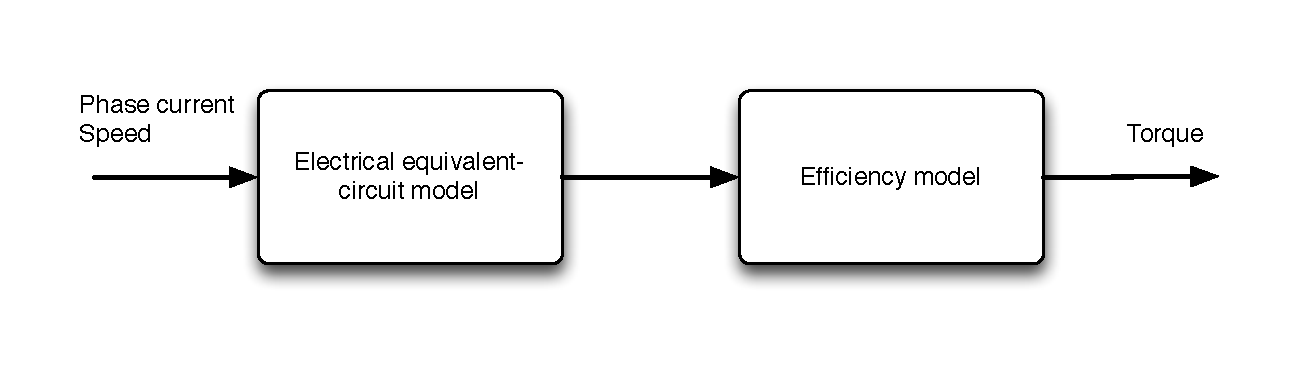
\includegraphics[width=\linewidth]{../Model/Powertrain/Motor/Documentation/Figures/Motor_block_diagram}
	%		\caption{Motor controller model block diagram.}
	%\end{figure}
	%\FloatBarrier

\section{Inputs and outputs}
	\subsection{Inputs}
	\begin{tabular}{ r | c | l | l }
		Signal						&	Symbol				&	MATLAB variable				&	Unit						\\\hline	
		Commanded motor current		&						&	\texttt{Motor\_Current\_Command}	&	\%					\\
		Commanded motor velocity		&						&	\texttt{Motor\_Velocity\_Command}	&	rpm			\\
		Commanded DC bus current		&						&	\texttt{Bus\_Current\_Command}	&	\%			\\
		Motor speed					&	$\omega_m$			&	\texttt{omega\_m}				&	rad/sec		\\
		Motor temperature				&	$T_m$				&	\texttt{T\_m}					&	\degree C		\\
		DC bus voltage				&	$V_\text{dc}$			&	\texttt{Vdc}					&	V
	\end{tabular}
	
	\subsection{Outputs}
		\begin{tabular}{ r | c | l | l }
			Signal						&	Symbol				&	MATLAB variable	&	Unit						\\\hline	
			Motor q-axis current			&	$I_q$				&	\texttt{Is.Iq}		&	rms amps			\\
			Motor d-axis current			&	$I_d$				&	\texttt{Is.Id}		&	rms amps
		\end{tabular}
	
\section{Background, rationale, modeling strategy}
	The motor controller model is actually two separate models: the motor controller, which makes control decisions based on rider commands and sensor feedback; and the power inverter, which is responsible for power conversion between DC and three-phase AC power.
	
	For this model, a simplified motor controller was developed based on documentation and working knowledge of the Tritium WaveSculptor 200, a commercially available unit used by the team. The power inverter was modeled as a lossless feedthrough pending the availability of efficiency data.
	
	\subsection{Motor control}
		A number of strategies for permanent-magnet synchronous motor (PMSM) control are available. Most modern strategies are based on space-vector control using the Park reference frame transformation \cite{Park1929}. At their core, these strategies have the goal of determining the magnitude and phase of the motor current that should be used to achieve a given torque value.
		
		The WaveSculptor 200 uses so-called "$I_d = 0$" control, where the phase angle between the motor's back-emf and the motor phase current is controlled to zero. In the most common configuration, the the rider throttle input is mapped linearly to the motor torque command, which in turn is mapped linearly onto total motor current.
		
		\begin{equation}
			I_s = I_{s,max} \times (\text{Rider throttle command})
		\end{equation}
		
		
\section{Parameters}
	
	\renewcommand{\arraystretch}{1.5}
	\begin{tabular}{ p{5cm} | c | l | l }
		Parameter					&	Symbol				&	MATLAB variable	&	Unit						\\\hline	
		Q-axis inductance				&	$L_q$				&	\texttt{Lq}			&	H			\\
		D-axis inductance				&	$L_d$				&	\texttt{Ld}			&	H			\\
		Equivalent-circuit series resistance	&	$R$					&	\texttt{R}			&	ohm			\\
		Permanent-magnet flux linkage	&	$\phi_m$				&	\texttt{phi}		&	V s $\text{rad}^{-1}$	\\
		Motor efficiency				&	$\eta$				&	\texttt{eta}		&				\\
		Motor efficiency lookup: stator current breakpoints	&			&	\texttt{eta.Is}		&	rms amps ($I_s$)	\\
		Motor efficiency lookup: motor speed breakpoints	&			&	\texttt{eta.omega}	& 	rad/sec		\\
		Motor efficiency data			&						&	\texttt{eta.eta\_m}	&	
	\end{tabular}


\section{Assumptions}
	The motor electrical model is significantly simplified.
	\begin{itemize}
		\item 
			The model assumes that the motor magnetization is linear (i.e., the motor never saturates).
		\item
			The model assumes that the motor inductances $L_d$ and $L_q$ are constant. In fact, \todo{details about behavior of Lq with Id}
		\item
			The motor efficiency model assumes that motor efficiency $\eta$ depends only on motor speed and electrical torque.
	\end{itemize}

\bibliographystyle{plain}
\bibliography{bib/SimBALink}

\end{document}